\documentclass[letter,12pt]{article}
\usepackage[letterpaper,right=1in,left=1in,top=1in,bottom=1in]{geometry}
\usepackage{setspace}

\usepackage[utf8]{inputenc}   % allows input of special characters from keyboard (input encoding)
\usepackage[T1]{fontenc}      % what fonts to use when printing characters       (output encoding)
\usepackage{amsmath}          % facilitates writing math formulas and improves the typographical quality of their output
\usepackage[hyphens]{url}     % adds line breaks to long urls
\usepackage[pdftex]{graphicx} % enhanced support for graphics
\usepackage{tikz}             % Easier syntax to draw pgf files (invokes pgf automatically)
\usetikzlibrary{arrows}

\usepackage{mathptmx}           % set font type to Times
\usepackage[scaled=.90]{helvet} % set font type to Times (Helvetica for some special characters)
\usepackage{courier}            % set font type to Times (Courier for other special characters)

\usepackage[longnamesfirst, sort]{natbib}\bibpunct[]{(}{)}{,}{a}{}{;} % handles biblio and references 

\usepackage{rotating}         % sideway tables and figures that take a full page
\usepackage{caption}          % allows multipage figures and tables with same caption (\ContinuedFloat)

\usepackage{dcolumn}          % needed for apsrtable and stargazer tables from R to compile
\usepackage{arydshln}         % dashed lines in tables (hdashline, cdashline{3-4}, 
                              %see http://tex.stackexchange.com/questions/20140/can-a-table-include-a-horizontal-dashed-line)
                              % must be loaded AFTER dcolumn, 
                              %see http://tex.stackexchange.com/questions/12672/which-tabular-packages-do-which-tasks-and-which-packages-conflict


\newcommand{\mc}{\multicolumn}

%% TO ADD NOTES IN TEXT, PUT % BEFORE THE ONE YOU WANT DISABLED
\usepackage[disable]{todonotes}                            % no show
%\usepackage[colorinlistoftodos, textsize=small]{todonotes} % show notes
\newcommand{\emm}[1]{\todo[color=red!15, inline]{\textbf{Eric:} #1}}
\newcommand{\vp}[1]{\todo[color=green!15, inline]{\textbf{Vale:} #1}}
\newcommand{\ges}[1]{\todo[color=blue!15, inline]{\textbf{Ges:} #1}}

\usepackage{xr} % allows cross-ref to other file
\externaldocument{urge15appendix}

%% %for submission: sends figs, tables, and footnotes to last pages
%% \RequirePackage[nomarkers,nolists]{endfloat}     % sends tables and figures to the end
%% \RequirePackage{endnotes}                        % turns fn into endnotes; place \listofendnotes where you want 
%%                                                  %the endnotes to appear (it must be after the last endnote).
%% \let\footnote=\endnote
%% \newcommand{\listofendnotes}{
%%    \begingroup
%%    \parindent 0pt
%%    \parskip 2ex
%%    \def\enotesize{\normalsize}
%%    \theendnotes
%%    \endgroup
%% }
%% 
%% % for submission: drop page numbers when producing title page
%% \pagenumbering{gobble} % Remove page numbers (and reset to 1)
%% \pagenumbering{arabic}% Arabic page numbers (and reset to 1)


\setcitestyle{citesep={;}}

\usepackage{listings}

\begin{document}

\title{Speech in Mexico's Cámara de Diputados\thanks{Financial support ITAM, SNI. For shedding light on some parties' internal rules of debate in the period, I am grateful to Fernando Rodríguez Doval, Lupita Vargas Vargas, and one former deputy who wished anonymity. Vidal Mendoza, Eugenio Solís, Sonia Kuri K, ana lu for research assistance.}}
\author{Eric Magar \\ Instituto Tecnológico Autónomo de México}
\date{\today}
\maketitle

%\newpage

\begin{abstract}
\noindent Text as data: speeches in lower chamber of Mexico's federal Congress. Analysis covers three pre-midterm election legislative terms since 2006. Argument, findings.\footnote{{Data and supporting materials necessary to reproduce the numerical results in the article are available in the following repository (\url{https://github.com/emagar/legdeb}). Supplementary material for this article is available in the appendix in the online edition.}}
\newline
\newline
\textbf{Keywords}: Speech, Congress, presidentialism, Mexico 
\end{abstract}

%\newpage

\doublespacing

\section{Introduction} [max 500 words]
%% -describe what the chapter is about, key findings, and distinctive features of the country

Interest in the Mexican Congress arrived with democratization.

Was more or less a rubber stamp, presidential super-majorities.

Then came divided government. Constitutional powers scrutinized, descriptive studies of relative influence by president, his party, and opposition parties. Roll call voting = cohesion, gubernatorial influences.

Debate has been overlooked. I could find no reference to anything. Chapter explores. Institutions and members' access to the floor to deliver speeches.

Argument. 

\section{Case selection}

Due to a hard time constraint, I leave out the Senate from analysis and focus on three out of eight Cámara terms since democratization. I examine the 60th (2006-09), 62nd (2012-15), and 64th Legislatures (2018-21). All are pre-midterm election terms for comparability. Data for the 64th runs up to the end of the second ordinary year only (March 19th, 2020, with more than one full year remaining), enough to investigate effects of electoral reform and majority status in debate, as we will see. 

%I had to limit data span due to a hard time constraint. Focus is on the Cámara de Diputados only. The chambers of the bicameral Congress have symmetric powers over most legislation, but the Senate is excluded from adoption of the annual budget, and I left it out. The limit is also in the time span. Only three legislative terms out of eight since democratization are included. I examine the 60th, 62nd, and 64th Legislatures. All are pre-midterm election, more similar among them. I opted for inclusion of the partial 64th Legislature (2018-21) instead of the 58th (2000-03) in order to investigate effects of electoral reform in debate. 


\section{Institutional and party system background} [ca 500-1000 words]
%% In this section, you need to address the basic institutional design of your country.
%% Please cover, at least, the following points:

Mexico is a presidential democracy. For most of the 20th century a hegemonic party, the PRI, held the strings of political influence in a tight grip nationwide. While the PRI's electoral fortunes suffered from societal change \citep{scott.1959}(ref) and from formidable economic setbacks in the 1980s, it was not until 1997 that competitive politics became the norm. The PRI lost control of the lower house of Congress in that year's midterm election, the first in six decades. Then in 2000 the country's long-standing right-of-center opposition beat the PRI in the presidential race. 

Congress is bicameral. The only asymmetry in the chambers' authority over legislation is important: the Cámara de Diputados adopts the federal budget without Senate intervention. 

64 partial included because it is the first instance of single-party unified government. And, importantly, first Congress where incumbents allowed to be on the ballot in midterm. Plus clear mutation of governing groups after 2+ decades of the partidocracia party system \citep{magar.2007ref.2015,magar.estevez.rosas.2010}. 


Mexico has a presidential constitution. For most of the 20th century a hegemonic party, the PRI, controlled the strings of political influence nationwide. While the PRI's electoral fortunes suffered from societal change and from formidable economic setbacks in the 1980s, it was not until 1997 that competitive politics became the norm \citep{cosio.villegas.1981,molinar.1991a,cornelius.1996}. The PRI lost control of the lower house of Congress in that year's midterm election, something unseen in over six decades. Three year later the country's long-standing right-of-center opposition, the PAN, beat the PRI in the presidential race. 

%% 1. Describe the institutional system: executive-legislative relations; balance of power between executive and legislative branches. Does the executive dominate?

With democratization, two decades of divided government ensued. The executive's control of the legislative process ended abruptly, inaugurating relative balance between the branches \citep{weldon.1997,lujambio.segl.2000}. The president retained a prominent role in lawmaking, but genuine negotiation with the opposition was required to get things done \citep{casarSinMay2013,bejarQuienLegisla2012}. 

%% 2. Parties and party system: describe the most important parties in the window of observation of the chapter. Discuss party system features. Are there dominant parties? Are there extreme left or right parties? Are the latter considered outsider parties?

Competitive politics blended a
- three party system (local two-party systems mostly) with 
- entry barriers
- but weak links to society
- bunch of opportunistic parties
- two dims of competition

Partidocracia came crashing down in 2018.

  \subsection{parties in camara}

\singlespacing
\begin{footnotesize}
\begin{verbatim}
|----------------------------+------+------+--------|
|                            | 60th | 62nd |   64th |
| party                      |    % |    % |      % |
|----------------------------+------+------+--------|
| pan                        |   41 |   23 |     16 |
| pri                        |   21 |   43 |      9 |
| prd                        |   25 |   20 |      4 |
| morena                     |      |      |     51 |
| opportunistic w/ president |      |    8 |     14 |
| other opportunistic        |   13 |    7 |      6 |
|----------------------------+------+------+--------|
| Total                    % |  100 |  100 |    100 |
|                          N |  500 |  500 |    500 |
|----------------------------+------+------+--------|
| president's party          |  pan |  pri | morena |
|----------------------------+------+------+--------|
\end{verbatim}
\end{footnotesize}
\doublespacing

%% |              |  60 |  62 |     64 |
%% |              |   N |   N |      N |
%% |--------------+-----+-----+--------+
%% | pan          | 207 | 114 |     79 |
%% | pri          | 104 | 213 |     47 |
%% | prd          | 125 | 102 |     20 |
%% | morena       |     |     |    255 |
%% | opport w pdt |     |  38 |     69 |
%% | oth opport   |  64 |  33 |     30 |
%% |--------------+-----+-----+--------+
%% | Total        | 500 | 500 |    500 |


%% 3. Discuss the organization of parliamentary party groups/legislative parties. The balance of power between frontbenchers (leadership) and backbenchers.

Mandarins quote here. Frontbenchers pull the strings. Single-term limits with centralized nominations. Will change in 2021. 

%% 4. Electoral system: discuss personal vote-seeking incentives. Frame this in a way that answers the questions: is the electoral system party-centered or candidate-centered? Discuss existing empirical work about your country that deals with home style. Discuss the ballot structure and how it allows voters to reward/punish individual legislators. Conclude point by referring to the importance of the ‘party brand’ as an electoral asset? Is the party brand important for vote-seeking (e.g. in CLPR, such as Portugal, Spain or Norway) or is the party brand of less importance (e.g. in Irish STV)?

The Cámara's electoral system is mixed member plurality \citep{weldonMixedMemberSys2001}. Three-hundred members elect by first-past-the-post in single member districts (SMDs) and two-hundred members by closed-list proportional representation. All members have three year terms. All seats are contested in races that are concurrent with the presidential election, then again at the presidential midterm. 

Reliance in primaries for SMD candidate selection---mostly by the PAN \citep{ascencio.kerevel.cand-sel-beh.2021}, on occasions by the PRI \citep{poire.phd.2002}---opens some exceptions, but in general ballot access is controlled by national and state party leaders \citep{rosas.langston.2011,langston.2008}. With this feature, systems with SMDs (the large portion of the mix) and closed-list PR (the other portion) belong at the bottom of Carey and Shugart's \citeyearpar{carey.shugart.1995} ordinal rank of incentives to cultivate personal vote. 

Another feature of importance are single-term limits, which the constitution set on all elected officeholders. Ambition was perforce progressive \citep{schlesinger.1966} and centralized nominations acted as a potent agent for discipline to party leaders. But, in a surprising recent development, single-term limits were eliminated for selected offices, including federal deputies \citep{magarInstReel.2017}. The 2021 midterm election will be the first since the 1930s where incumbents will be allowed on the ballot.

Deputies elected in 2018 and hereafter have four-term limits instead. Reform should introduce a degree of personal vote seeking among a subset of deputies with static ambition. While reformers further centralized nominations by keeping the ban on consecutive reelection for party switchers in general, this might not fully reign in competitive incumbents: parties removing previous winners of elected office, dynastic candidates \citep{enriquez-dinastias2018itam}, and what \citep{zallerprizeFighters} refers to as "prize fighters", in order to secure nomination of docile newbies, risk losing those districts. I investigate effects of reform on debate. 

Another extraordinary event was the critical election of 2018, marking the demise of the three-party system that brought democracy. After decades of infighting the left finally split. The faction loyal to AMLO successfully launched a new party, Morena, overcoming formidable entry barriers \citep{magar.2007ref.2015}, a feat that placed his in the way of winning the presidential election by a landslide. For the first time in over two decades, the president's party enjoyed majority status in Congress. The effects of electoral reform and party system change, inf any, will be confounded...

%% 5. How important is party unity/cohesion for electoral success? Do institutional rules make party leaders value unity or can they allow MPs to dissent?

Unclear in past. Reelection should change things, incumbency times static ambition should matter more. Mention candado partidista? 

\section{The institutional setting of legislative debate in the Cámara} [ca 1500 words]

%% In this section, we need to set the rules of the game for legislative debates. As we have seen in our workshop, there is a high heterogeneity in the institutional setting of legislative debates. Producing a thorough discussion of formal and informal rules across a wide-range of countries is a valuable contribution of the volume to the discipline. Please try to answer the following questions in your country chapter:

%% 1. Who can allocate speaking time to individual MPs? Who controls the legislative agenda – government, parties, MPs, some legislative structure specifically in charge with agenda-setting? In answering this question, you should aim to discuss both formal rules (constitutional rules, rules of procedure), party internal rules (if they exist), and informal rules.
%% 2. Do individual MPs have a guaranteed right to participate in a debate without party leadership permission? If yes, how much time and in which type of debate? 
%% 3. How is the debate structured? What are the rules of engagement? Do MPs engage in back-and-forth talk? By contrast, do MPs deliver a debate without interruptions?
%% 4. Do particular subsets of MPs (e.g. spokesperson or committee members) have formal rights that entitle them to take the floor?
%% 5. What are the existing types of debates? Please select the 5 most important types of debates and produce a table where you cover the name of the debate (in English and the native language of the country), its goals, particular organization rules to that kind of debate, and the total number of minutes that rules assign to each debate.

%% To conclude this section, please classify the country along Proksch and Slapin’s (2015) contribution. The authors suggest that there are two extreme poles, depending on rules of procedure and electoral system organization. As described by Proksch and Slapin (2015: 96), in some systems, individual MPs are ‘guaranteed access to speaking time’, and ‘backbenchers are granted equal time as party leaders’. In other systems, the rules severely restrict individuals’ access to the floor and parties draft speakers lists, which gives party leaders much more control on this question. A number of countries fall, however, somewhere between these two extreme categories, giving some opportunity for individual MPs to access the floor, but favoring party lists. Please classify your country accordingly. If your country was included in Proksch and Slapin’s study, please refer to this classification when discussing your country’s institutional setting.


An overview of the structure of legislative debate shows members who have abdicated most formal speech rights to their parties. The Cámara's Rules \citep{reglamentoDipMx.2019} set most prescriptions for debate, with general guidelines in Congress' Organic Law \citep{loceum.2019}.

\citet{casar.agsetting.2016} examination of agenda setting puts the focus on results (passage of legislation). Her mention to debate characterizes it as party-centered: "[governing] bodies have the power ... to conduct floor debates, including assigning turns and time to speakers" (p. 154). This, we will see, is not in alignment with formal institutions, which establish individual member rights to be recognized by the presiding officer.

Proksch/Slapin here? the apradox is explained by parties... 



  \subsection{The boards}
There are two key actors in the legislative process, the Junta and the Mesa. The *Junta de Coordinación Política* is the Cámara's top decision-making organ. The leaders of all parties with no fewer than five deputies are represented. The majority leader presides the Junta throughout the term. In the absence of a majority party, however, the leaders of the top-three seat holding parties preside the Junta, alternating one year each. The Junta appoints and replaces committee members, prepares each session's order of the day (/orden del día/), and in general reaches and enforces party leader agreements. It decides by majority rule, with members' votes weighted relative to group sizes in the plenary. So majority status is crucial to control the Junta \citep[cf.][]{cox.mccubbins.2005}.

%One is the *Cámara president*, an officer similar to the Speaker in the UK House of Commons. Diputados are expected to address the chamber president, who is responsible for keeping debate orderly and within chamber and congressional rules. Other officers are secretarios, responsible for formalities such as reading bills, committee reports, or other motions presented to the plenary for consideration, announcing the result of roll call votes, an so forth.  


The *Mesa Directiva* is the chamber's steering board. The Mesa chair is the Cámara president ex-officio. The Mesa makeup has consensual traits, regardless of there being a majority party or not. It is elected yearly by two-thirds supermajority of Cámara members from candidates proposed by the Junta. While Mesa members can reelect, the chair must rotate between the top-three seat-holding parties, one year each. 

%The president recognizes speechmakers and presides over Cámara debates. The Mesa includes deputy presidents and at least one secretary from each parliamentary group. The Mesa follows the session's agenda in the Day's Order (/Orden del Día/) that is mostly set by the Junta. 

% I use the terms party and parliamentary group interchangeably, but groups are in fact more restrictive. A group (/grupo parlamentario/) needs no fewer than five deputies to earn and retain Junta representation. Moreover, groups can only form at the term's outset. Members can freely leave one group and may join another existing group at any time, with immediate effects in vote weights. But defectors cannot form new groups---no doubt raising the cost of lone turncoats. 

Agenda control is frail. First, every committee report is guaranteed floor consideration and must be included in the order. If committees were adequate agents of the Junta majority, they might serve as gatekeepers by denying unwanted bills a report. But the Junta is required to distribute committee chairs (as well as committee seats) proportionally among the parties, so some committees are bound to be preference outliers.

Second, the open rule is the default for bill consideration in the floor. Debate takes place in two stages. The entire bill is first examined /en lo general/, then articles are considered individually for amendment or deletion /en lo particular/ \citep[see][]{heller.weldon.nd}. Members can always reserve articles for deletion or amendment, denying the Junta a useful procedural tool common in other assemblies: the closed rule \citep[eg.,][]{cox.2006,weingast.1992,magar-palanza-sin-Pdt-fast-track-chile-2021jop}.

Third, and most relevant, speakers can self-select. Individual members are entitled to take the floor when recognized by the presiding officer, for a duration set by rules or by party agreements. Party leaders allocate speaking time to a list of speakers but cannot preclude others from adding their names to that list, making debate resemble first-come-first-serve once parties have spoken. 

%%Formally, deputies enjoy equal rights and duties. With respect to deliberation, all are entitled to take the floor when recognized by the presiding officer, for a duration set by rules or by party agreements. However, as in assemblies worldwide, members with status tend to have many more rights, the rest many more duties. What defines status changes from one assembly to the next \citep{cox.2006}. In the Cámara, party leaders in general, and majority party leaders in particular sit atop the status pyramid. But when it comes to speech, individual members retain debate rights that set the basis for minority rights. 

  \subsection{The structure of debate}
Rules set limits for different kinds of debate summarized in the Table. The first entry refers drafters of new legislation, who who get first recognition to take the floor in order to persuade fellow lawmakers. The time limit is ten minutes when the draft is a new law, five minutes when it amends existing statutes. Deputies who wish to debate then get five minutes each. Bills that cannot be presented before the session ends migrate to the next day's order upon author's request /viva voce/ (otherwise they are referred to committee.) The rightmost columns report who selects the speaker---self-selection by drafting a bill, in this case---and who, if anyone, can veto the speaker's recognition---no one here. 

\begin{table}
  \begin{scriptsize}
    \begin{verbatim}
|----------------------------------------+---------------+---------+------------+------------|
| Debate type (in Spanish)               | Goal          | Durat.  | Selector   | Veto       |
|----------------------------------------+---------------+---------+------------+------------|
| 1. Introduce legislation (iniciativa)  | Author        |         |            |            |
| - a new law                            | presents      | - 10'   | - member   | - no       |
| - amend a law                          | the bill      | - 5'    | - member   | - no       |
|----------------------------------------+---------------+---------+------------+------------|
| 2. Committee report (dictamen)         | Move          |         |            |            |
| - Debate en lo general vs SQ, chair    | for floor     | - 10'   | - comm.maj | - pres.^1  |
| -   "             "      "   others    | consideration | - 5'    | - members  | - pres.^1  |
| - Amendments (debate en lo particular) |               | - 5'    | - members  | - no       |
| - negative report                      |               | - 3'    | - comm.maj | - pres.^1  |
|----------------------------------------+---------------+---------+------------+------------|
| 3. Resolutions (puntos de acuerdo)     | Position      |         |            |            |
| - standard, author                     | taking        | - 10'   | - member   | - comm.maj |
| - urgent, author (obvia resolución)    |               | - 5'    | - Junta    | - floor    |
| - other speakers                       |               | - 3'    | - party    | - no       |
|----------------------------------------+---------------+---------+------------+------------|
| 4. Current events (agenda política)    | Position      | < 2hrs  |            |            |
| - Junta proponent                      | taking        | - 10'   | - Junta    | - no       |
| - other speakers                       |               | - 5'    | - member   | - no       |
|----------------------------------------+---------------+---------+------------+------------|
| ^1 = President can delay/prevent speech by granting recommit.                                |
|--------------------------------------------------------------------------------------------|
\end{verbatim}
  \end{scriptsize}
\caption{Types of debate}
\end{table}

Other speech types grant right of first recognition differently. Debate /en lo general/ grants it to the reporting committee chairperson or designated handler of the report for ten minutes (fifteen in constitutional amendments). The Cámara president can delay debate by recommitting the bill---and possibly prevent it if the committee kills the bill. /En lo particular/ amendments and Cámara resolutions grant it to the proposing member. 

Party-appointed speakers get five minutes each, in reverse-size order, after the first /en lo general/ speech. Then members who request it then get five minutes each, the president arranging them in rounds, one for one against. After six such rounds, the floor can either proceed to vote, or continue with blocks of three such rounds. When the report deals with issues of great interest, debate can go on for several hours.

%Floor (108) must approve member requests to consider an article separately from general discussion (deletion amendment?)

%Votos en lo particular = another window for dissenters. Minority report. Minority reports get floor consideration only when floor rejects the committee report. 

%Discusión en lo particular = introduce amendments to committee report (who can do it? who can block? 110 silence suggests that any member can do it --- open rule unless rules are suspended?) Proposer gets 5 minute speech, then for/againsts get 5 minute each.

Cámara resolutions (/proposiciones con punto de acuerdo/) are tailor-made for members' position-taking needs, conditional on party leader support. If adopted, resolutions become the opinion of the chamber on some specific issue. But they require urgent status (/urgente u obvia resolución/) in order to avoid committee referral and move directly to the floor; only the Junta can request that the floor grants urgent status to at most two resolutions per session. If granted, the proposer takes the floor for five minutes. Parties then appoint one speaker each, for three minutes. The floor can then decide to vote, or open a rounds of debate with self-appointed speakers.

Current events (/agenda política/) are party leaders' position-taking venue. The Junta determines up to two themes for debate before consideration of reports and bills, party leaders appointing one speaker each. The promoting party speaker gets first recognition for 10 minutes, others 5 minutes each, and talk in reverse-size order. Current events debate cannot exceed two hours per session. 

  \subsection{Recognition-granting motions}
Debate under such rules becomes a succession of punctuated, mostly uninterrupted short speeches. Members can approximate back-and-forth talk, at least occasionally, by catching the president's eye from their seats in order to interrupt with a motion. The president has discretion to deny, or grant up to three minutes to elaborate. Such motions are distinct from points of order (which members can also make, see Reglamento art. 114 for typified motions). They grant recognition to speak. One (/cuestionamiento al orador/) to interrogate the speaker, who must also accept the question be made. Another is (/alusiones personales/), to give right of reply to alluded members by recognizing them right after the speaker ends. And (/rectificación de hechos/) wind up an additional name at the end of the list of speakers. 

  \subsection{Party discipline as alternative to centralized agenda power}
The Cámara's debate rules are ill-designed to prevent plenary bottlenecks \citep{cox.2006}. Even in the presence of a majority party, individual members retain speaking rights that water down attempts by the Junta to cartelize the legislative process. So how does the Cámara prevent dilatory motions to get things done? The answer is parties. Party discipline operates as an alternative to agenda cartelization in many systems \citep{prata.2006}. 

Cohesion is near perfect across parties. \citet{tellez-del-rio.2018} computed frequencies with which deputies voted against a majority of their party (excluding unanimous votes). The mean he reports for the 1997--2018 period stands at 2 percent, 3.4 percent when abstentions are coded as votes against the party majority (p. 25). 

Three former deputies from the larger parties offered quick impressions on internal party speech rules upon request. One commonality (at least in this very small sample) is the informal erosion of formal individual members' debate rights in favor of centralized speech allocation \citep[cf.][]{cox.1987}. The PAN relies on a debate whip (subcoordinador de debate parlamentario) in charge of selecting speakers in debates. When two members wish to speak at once, the whip would let them figure who would get the party's slot in the debate, who would then speak for or against.\footnote{Email exchange with Fernando Rodríguez Doval, June 17th, 2020.} The PRI leadership sets apart issues of party interest, appointing every speaker when debated. Members would communicate their wish to speak on unwhipped issues to their state caucus leader, who would seek authorization with party whips.\footnote{Email exchange with Lupita Vargas Vargas, June 17th, 2020.} Rules give parties one speaking slot each in many debates, regardless of size. Distributive conflict over speech is therefore more acute for larger parties, with longer speaker lists. A must for a member dissenting from ``party mandarins'' is a solid knowledge of the Rules. That member can thus make individual speaking rights effective by introducing suspensive motions or amendments, both of which come equipped with recognition to take the floor./footnote{Email exchange with a former deputy from the left, who answered on condition of anonymity, June 17th, 2020.} 

Party leaders move the strings of lawmaking. Their influence, however, derives almost exclusively from party discipline (near-perfect across the board) and not from agenda power (which is quite diffuse). 

  \subsection{Continuum}

Proksch and Slapin's \citeyearpar{proksch-slapin2015book} scheme, used across chapters in this volume, compares assemblies according to how members gain access to take the floor in order to deliver speeches (p. 79). A continuum connects two extremes: party-controlled access and individual member-controlled access. Formal rules place the Cámara towards the individual member-controlled access limit of the continuum; but partisan rules pull it towards the party-controlled access side. The removal of single term limits ought to make this tension between formal and de facto institutions harder to manage for all parties.  

(EMM quizás debo conectar continuum y bottlenecks/minority rights en seccióm Mexico?)

  \subsection{Minority rights}

Arg here: While parties sit atop the status pyramid, their agenda power is relatively limited. 
Two problems: can't easily prevent unwanted speeches as members retain right to talk; can't easily remove unwanted motions as committee reports proceed automatically to floor discussion. So negative agenda power is diffuse. 
Parties in fact rely on discipline towards leadership to avoid plenary bottlenecks and get legislation done. 

suspension of rules typified only for discharge, two-thirds

The constitution sets the quorum at half chamber membership.

Reglamento amendments by 2/3 vote

Suspension of rules by Conferencia always a choice, but only typified for committee of the whole. Art 77 cpeum. Risks toma de tribuna.

Presiding officer can summon police to restore order. 
Can summon public force, but in practice never used. 
Can kill the mike, but others can raise their voices

4. Para atender una situación no prevista en el Reglamento, el Presidente podrá dictar una resolución de carácter general, siempre que haya la opinión favorable de la Mesa Directiva y de la Junta. En caso contrario, este tipo de resoluciones sólo tendrán efecto con la aprobación de la mayoría simple del Pleno.

\section{The role of intra- and interparty politics in legislative debates?} [ca 2500]
 
  %% In this empirical section, we want you to explore how intra and interparty, as well as individual features, play a role in determining the likelihood that MPs take the floor (and how often they will take the floor). 
%% The section is divided into subsections. The first uses descriptive statistics and bivariate analysis. The second turns to multivariate analysis. 
%% Please note that the contents of this section are rigid. Please save important aspects that are relevant to your case to a subsequent section on ‘Country Specific Matters’. 

  \subsection{Data and The dependent variable}

Digitized speeches come from the stenographic service (scraped from http://cronica.diputados.gob.mx/). I relied on regular expressions to de-htmlize the text and identify speakers and their speech, turning text into data for analysis.\footnote{Data analysis was performed in R \citep{r.cite}, all code is available at https://github.com/emagar/legdeb. I relied on libraries lme4 \citep{r.lme4}, lubridate \citep{r.lubridate}, margins \citep{r.margins}, MASS \citep{r.mass}, plyr \citep{r.plyr}, stargazer \citep{r.stargazer}, and zoo \citep{r.zoo}.}

The *dependent variable* is a member's participation in plenary debate during legislative periods (see the appendix for terminology). The 60th, 62nd, and 64th Legislatures had six, eight, and five periods, respectively, totaling nineteen. Three are extraordinary periods, the rest ordinary. Mean days per period was 6.7 for the former, 31.4 for the latter, so the debate models control for period length. 

I use two specifications of the dependent variable, one absolute, one relative. The absolute is *words(i,p)* equal the number of words that member i spoke in period p. Days when deputy i spoke fewer than 50 words are arbitrarily considered non-debate and dropped, adding zero towards the member's aggregate. Since officers do not participate in legislative debate, all steering speech, as when the president recognizes a deputy or the secretary calls a voice vote to dispense reading of the bill, was also removed. So was speech by non-deputies, as in cabinet member hearings. Everything remaining is considered debate, members' daily totals added across sessions in the same period to produce aggregates for analysis.

The relative specification is *words(i,p)/exposure* equal the absolute words divided by the days that member i served as a proportion of all session days in period p (members can take leaves of absence). So the denominator for a member who spoke 2 thousand words and served uninterrupted throughout period p is one, and both specifications are equivalent. If she had served only half of the period instead, then the denominator would be 0.5, making her relative words equal 2000/0.5=4000 in that period. 

%As in other chapters, the dependent variable is the number of words that members spoke in the chamber. A given diputado's words throughout a plenary session were summed into a daily total. Daily totals less than 50 words were arbitrarily interpreted as not constituting speech and removed from the data (ie., the member received a value of zero words that day). Thus filtered, members' daily totals were added across sessions in the same period, producing word aggregates for analysis.

Table \ref{T:descriptives} has a summary of the dependent variable along others of interest. Member-period observations total 9494. The median member spoke 593 words per period, 607 when measured relative to days in office. At nearly 1400 words per period, means are substantially higher owing to a right-skewed speech distribution portrayed in Figure \ref{F:dv-hist}. Relevant to the choice of estimation methods, data appear to be over-dispersed (the standard deviation doubles the mean), so negative binomial appears the method of choice over poisson regression; and the nearly two out of five members who uttered not a single word in the period (37.6 percent) suggest adoption of a zero-inflated approach.

\begin{table}
  \begin{scriptsize}
    \begin{verbatim}
Part A: Continuous variables
|                              |   min | median |  mean |     sd |   max |    N |
|------------------------------+-------+--------+-------+--------+-------|------|
| Total words (DV1)            |     0 |    593 |  1366 | 2682.3 | 50291 | 9494 |
| Total words / exposure (DV2) |     0 |    607 |  1391 | 2716.3 | 50291 | 9494 |
| Days in office (exposure)    |     1 |     30 |  26.7 |   11.2 |    40 | 9494 |
| Party share                  |   0.4 |     25 |  29.2 |   15.9 |    51 | 9494 |
| Seniority                    |     0 |      1 |   1.7 |    2.2 |    17 | 9494 |
| Previous terms               |     0 |      0 |   0.3 |    0.6 |     4 | 9494 |
| Age                          |    21 |     46 |  45.9 |   10.1 |    78 | 7332 |


Part B: Dichotomous variables
|          |    0 |    1 | tot |    N |
|----------+------+------+-----+------|
| Spoke    | 37.6 | 62.4 | 100 | 9494 |
| Majority | 86.6 | 13.4 | 100 | 9494 |
| Leader   | 98.3 |  1.7 | 100 | 9494 |
| Chair    | 90.6 |  9.4 | 100 | 9494 |
| SMD      | 39.3 | 60.7 | 100 | 9494 |
| Suplente | 94.2 |  5.8 | 100 | 9494 |
| Extraord | 84.5 | 15.5 | 100 | 9494 |
| Female   | 64.2 | 35.8 | 100 | 9494 |
| 60th     | 68.2 | 31.8 | 100 | 9494 |
| 62nd     | 57.6 | 42.4 | 100 | 9494 |
| 64th     | 74.2 | 25.8 | 100 | 9494 |
| PAN      | 72.8 | 27.2 | 100 | 9494 |
| PRI      | 72.8 | 27.2 | 100 | 9494 |
| Left     | 70.0 | 30.0 | 100 | 9494 |
    \end{verbatim}
  \end{scriptsize}
\caption{Variable descriptives}\label{T:descriptives}
\end{table}

\begin{figure}
  \centering
    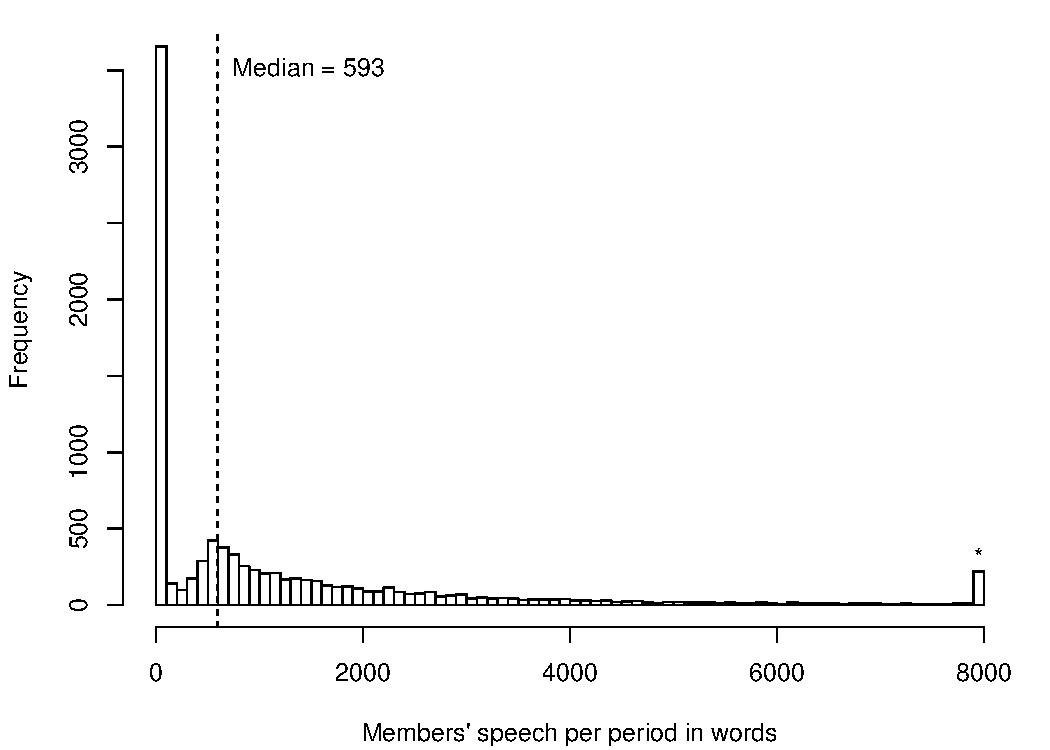
\includegraphics[width=.8\columnwidth]{../plots/dv-histogram.pdf}
    \caption{The dependent variable, absolute specification. The rightmost column under a star is fictitious, reporting 217 member-periods with 8 thousand words or more (2.2 percent of all, the actual distribution spreads these observations, with increasing sparseness, from 8000 to 50291).}\label{F:dv-hist}
\end{figure}

%% \begin{figure}
%%   \centering
%%     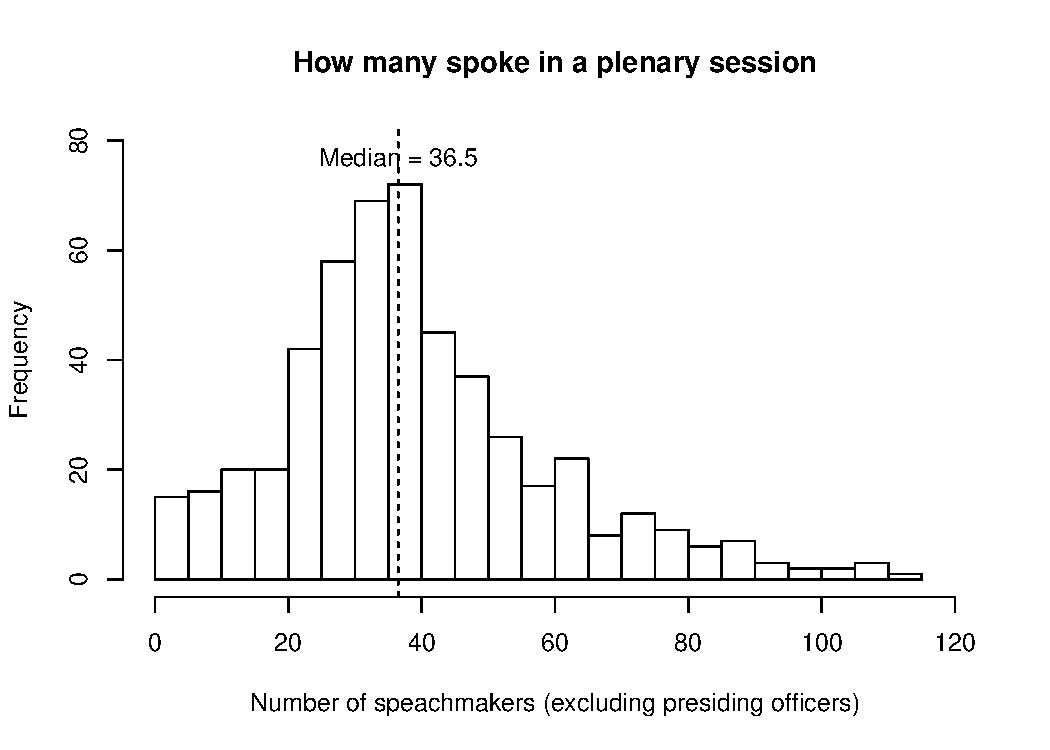
\includegraphics[width=.8\columnwidth]{../plots/nspeakers.pdf}
%%     \caption{Number of daily speakers}\label{F:nspeakers}
%% \end{figure}

Debate quantities are easier to grasp when expressed as daily totals instead of the period totals analyzed. In the median session, 36.5 different speakers contributed to daily debate, and six days had over 100 speakers. Figure \ref{F:quantiles} portrays member daily aggregates across the periods analyzed. For clarity, this plot includes speakers only (non-speakers are included in the period aggregates analyzed below.) Solid points report median daily speech length in words. With few exceptions, period medians are much the same as the overall median daily speech length of 599 words. Mild term effects show up too, the 60th medians slightly above and the 64th slightly below the overall median. Horizontal lines report the spread of the central portion of the density---the thicker line is the inter-quartile range, the thinner connects the first and ninth deciles. Period distributions are, in general, similar. The clearest exceptions are extraordinary periods, drawn in gray. The models therefore include controls for Legislature and ordinary session effects.

\begin{figure}
  \centering
    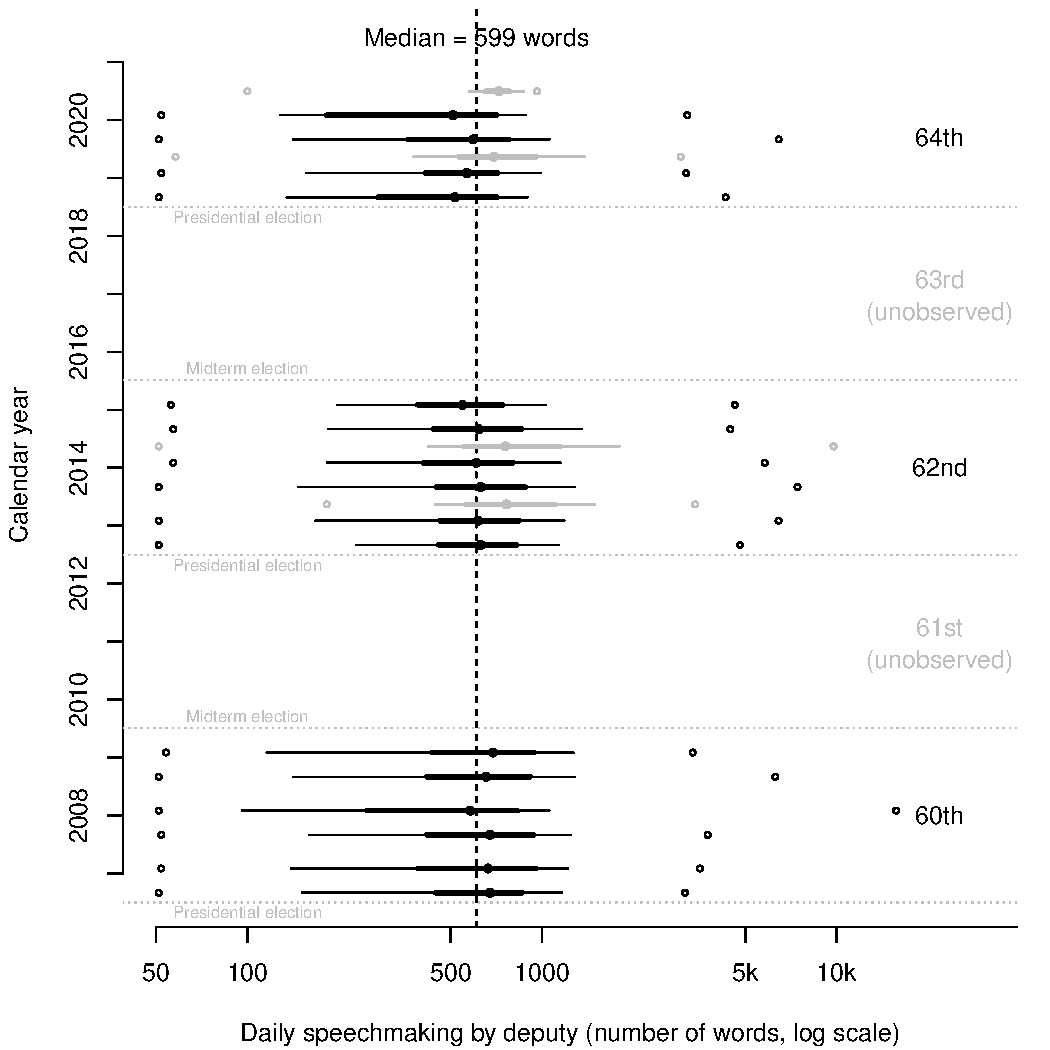
\includegraphics[width=.5\columnwidth]{../plots/quantiles-periodo.pdf}
    \caption{Daily speech length by legislative period observed. The plot excludes non-speaking members. Solid points indicate the median speech length in the period. Thick and thin lines connect the 25--75 and 10--90 percentiles, respectively. Hollow points are minima and maxima. Ordinary periods in black, extraordinary periods in gray.}\label{F:quantiles}
\end{figure}

Hollow points are minima and maxima. Diputada Valentina Batres holds the record for delivering the longest speech in the three terms examined. At 15,932 words, her speech delivered March 11th, 2008 is 50 percent longer than the runner-up and has about as many words as \emph{Don Quijote de la Mancha}'s chapters 1 through 7 (forty-five pages in the edition I own). Batres and legislators close to AMLO used dilatory tactics throughout that session, delaying the vote of a national geostatistics law. I suspect that filibustering was probably aimed at a bill down the line, with plainer distributive effects \citep[cf.][]{wawro.schickler.filibuster.2007}. A systematic study of filibustering in the Cámara is worthy of further study. The names associated with extreme member-periods (those grouped in Figure \ref{F:dv-hist}'s starred column to the right) are few: only nine deputies repeatedly surpassed 20 thousand words per period, mostly in the 62nd term. They are routine filibusters.
%Most are in AMLO's present government. 

%Sistema Nacional de Información Estadística y Geográfica
%Deputies close to AMLO were adoting dilatory tactics. Batres requested the addition of a point to JuCoPo's order of the day. Mesa Directiva denied, so a PRD faction threatened to take over the Tribuna (?). Batres introduced motion to suspend and other dilatory tactics (ley sis nal informacion inegi), then filibustered (called art. 103 ley reglamentaria, granting her 30 minutes to present minority vote despite JuCoPo's day aggreement to limit to 10 minutes.)

% Chapters 1 through 6 of El Quijote 13,049, 40 pages in my edition.
% Chapters 1 through 7 of El Quijote 14,916, 45 pages in my edition.
% Sonnets and Chapters 1 through 7 of El Quijote 16,191, 45+ pages in my edition.
% Chapters 1 through 7 of El Quijote 17,912, 45+ pages in my edition.

%The log scale magnifies the low side of the distribution. But it also blurs subtle but revealing differences in the high side. From 60th to 62nd, max went up while percentiles 75 and 90 remain at similar levels. Like Batres, an unusually high top decile consists of attempts to disrupt debate through filibustering. Dilatory tactics went down in 62nd compared with 60th, and substantially so in the 64th with a single party majority.


%% \singlespacing
%% \begin{footnotesize}
%% \begin{verbatim}
%% Words per day
%% | Legislatura    | min | 10% | 25% | 50% | 75% |  90% |   max |
%% | 60th           |  50 | 137 | 392 | 652 | 901 | 1215 | 15932 |
%% | 62nd           |  50 | 193 | 438 | 611 | 850 | 1254 |  9765 |
%% | 64th (partial) |  50 | 142 | 327 | 547 | 730 |  975 |  6358 |
%% \end{verbatim}
%% \end{footnotesize}
%% \doublespacing




  \subsection{Independent variables}

%% Please begin this subsection with a descriptive statistics table, including both DVs and all independent variables. Please include Mean, Std. Dv., Min, Max

%% Bivariate Analysis: Here, we cover two individual aspects. For each of these aspects, please produce a figure and discuss it. The editors will be sending you a do-file to harmonize the aspect of the figures across the volume. The following features should be discussed here:

%% 1. Gender: what is the impact of gender in floor access? Do women have access to the floor that is commensurate to their numerical presence in the legislative party? Operationalize gender as a dummy variable: Women takes the value of 1, and Men 0. Please use this coding also in the multivariate analysis (several drafts coded male MPs with 1 and female MPs with zero).

  Two quantities of interest across chapters are the intersections of gender and seniority with floor access. Of 1710 members observed, 39 percent are women. Owing to stricter quotas, 47 percent of the 64th Legislature members were women, up from 28 in the 60th \citep{piscopo.2016}. While disproportional among committee chairs and party leaders, the gender split among Cámara presidents is about proportional relative to women's numerical presence. So is access to the floor in terms of speakers (37 percent), but women are over-represented in terms of words (41 percent). Women delivered longer speeches.

\begin{table}
  \begin{scriptsize}
    \begin{verbatim}
|                   | % women |    of |
|-------------------+---------+-------|
| Members           |      39 |  1710^|
| -60th             |      28 |   603 |
| -62nd             |      41 |   640 |
| -64th             |      47 |   531 |
| Cámara presidents |      35 |    31 |
| Committee chairs  |      25 |   143 |
| Party leaders     |      21 |    24 |
| - major party     |       0 |    12 |
| - opportunistic   |      42 |    12 |
| Speechmakers      |      37 |  5926 |
| Words spoken      |      41 | 17.5M |
|-------------------+---------+-------|
|^Returning members counted once only.|
|-------------------+---------+-------|
    \end{verbatim}
  \end{scriptsize}
\caption{Women representation and debate}\label{T:women}
\end{table}

%% 2. Seniority: what is the impact of career stage in the likelihood of accessing the floor? Do more senior legislators get more access to the floor because they have offered party leaders signals of their work as party agents? Operationalize Seniority as a continuous variable that measures the number of years the MP has spent in the legislature.

Single-term limits offer little leverage to evaluate how seniority impacts floor access. Members wishing to return had to wait one term at least. Still, of 1710 members observed, 14 percent had previous federal deputy experiece. This suggests that the removal of single-terms will not be irrelevant due to lack of static ambition (as in Argentina, for instance). Freshmen spoke 1212 words on average in the period, compared to 1966 for members with one past term or more as deputies. Deputy-periods with one past term spoke 48 percent more words than those with none; those with two past terms spoke 61 percent more words than those with one; but members more than two past terms spoke 25 percent less words than those with two. This drop could be attributable to earlier recruitment of senior members, antedating competitve politics; or it could be due to the higher probability that senior members occupy leadership posts that might depress willingness to speak despite floor access possibilities. The multivariate analysis might shed some light.  


\begin{table}
  \begin{scriptsize}
    \begin{verbatim}
|  Past | Mean words | Member- |
| terms |  by period | periods |
|-------+------------+---------|
|     0 |       1212 |    7558 |
|   > 0 |       1966 |    1936 |
|     1 |       1796 |    1523 |
|     2 |       2892 |     330 |
|   > 2 |       1413 |      83 |
|-------+------------+---------|
    \end{verbatim}
  \end{scriptsize}
\caption{Seniority and floor access, member-periods}
\end{table}
  
  \subsection{A model of debate}

%% In this subsection, we run multivariate analysis explaining the determinants of participation in legislative debates. Before we go into the details of the analysis, let’s pause to discuss the unit of observation. As a rule of thumb, the unit of observation (each row in the data matrix) should be the MP over legislative term. However, some of you expressed the desire to have more disaggregated levels of analysis. For example, to observe the MP per day, MP per month, MP per legislative session. We are happy with the choice that you make, provided that you explain it in a clear way to help the readership making sense of it. 

%% In this section, we want you to run models using two different dependent variables:

%% 1. Number of speeches that a legislator delivered in the time unit you defined (presumably, for most of you, the legislative term). In doing so, use a negative binomial regression.
%% 2. Number of words divided by exposure (see below how to operationalize) that a legislator delivered in the time unit you defined (presumably, for the most of you, the legislative term). In doing so, use an OLS.
%% 3. For both cases, please included fixed-effects for the time period of interest (e.g., for the legislative term or the legislative session, depending on your choice). 
%% 4. Please include standard errors clustered at the legislator level.

%% What are the independent variables that you should use? As we talked over the workshop, in this section we need you to make models that are the same (or at least very similar) for all countries. In the country-specific section, you are free to make model extensions to account for country specification

%% In this section, please include the following covariates:

%% 1. Gender – dummy variable that takes a value of 1 for Women and 0 for Men
%% 2. Party Size – continuous variable that measures the absolute number of members of the legislative party
%% 3. Seniority – continuous variable that measures the number of years the legislator has been in the parliament
%% 4. Age
%% 5. Age Squared
%% 6. Party Family (Dummy variables, using one of party families as reference category)
%% 7. Committee Chair – dummy variable that takes a value of 1 if the MP holds a committee chair and 0 for all others
%% 8. Minister – dummy variable that takes a value of 1 if the MP is a minister and 0 otherwise
%% 9. Government party member – dummy variable that takes a value of 1 if the MP belongs to a legislative party that belongs the government and 0 otherwise. Note that we only consider parties that are formally in a coalition (i.e., have members in the executive). Supporting parties, e.g. contract parliamentarism, do not count towards government parties.
%% 10. Legislative Party Leadership – dummy variable that takes a value of 1 if the MP belongs to the leadership of the parliamentary party group
%% 11. Party Leader – dummy variable that takes a value of 1 if the MP is the party leader and 0 otherwise
%% 12. Exposure (logged) – continuous variable that measures the percentage of time in which the MP held to her seat in parliament during the unit of time defined in your chapter. For example, if you are using a MP-legislative term unit of observation, in this variable you need to include the percentage of time during the legislative term in which the MP was in the parliament. If MP was in parliament for whole session that would be 1. If the MP joined the parliament later, it could be .7 or .8. If you are using month as the time unit, the same rationale applies. The logged version should *only* be included in the count models (negative binomial). 

%% How to build the DV for the OLS models: 

%% Where the outcome is the number of Words, you should use Exposure as the denominator to create a ratio. The said ratio should consist of the "total number of words legislator i delivered during legislative term t/percentage of time legislator i sat in legislative term t”.

%% The rationale behind this measure is that we want to capture the time that each legislator sits in parliament during a given session. Obviously, a legislator who sits for the duration of the terms has higher chances of taking the floor than a legislator that takes her sit in the middle of the term.

%% Don’t forget to include Term FE, plus clustered standard errors at the MP level.

%% Please produce a table including both the negative binomial models and the OLS. For negative binomial models, please report the AIC.

%% Please include up to 5 models in the tables. Consider using a step-wise approach to regression by including covariates into the equation that make most sense in your context. 
%% Ultimately, we need 2 final models, where all variables are included – one where the dependent variable is the Number of Speeches and the other where the dependent variable is the Number of Words.

%% As a default we consider the following variables as explanatory:
%% 1. Gender
%% 2. Seniority
%% 3. Committee Chairs
%% 4. Minister
%% 5. Government party member
%% 6. Legislative Party Leadership
%% 7. Party Leader

%% The following variables are considered controls:

%% 1. Age
%% 2. Age Squared
%% 3. Party Family
%% 4. Exposure (logged)

%% Please feel free to use variables interchangeably between the two categories depending on the context. 

%% Please plot marginal effects using the full specification of the negative binomial model. In the said plot, please include explanatory variables only. Controls variables can be omitted.


To analyze participation in floor debates, I fit multivariate event count models to words spoken. In the right side are status variables, member characteristics, and controls. Units are member-periods. 

    \subsubsection{Status variables}

A dummy for *majority* status indicates members from Morena in the 64th Legislature---the only party controlling over 50 percent of seats. If debate is an (imperfect) substitute for legislative outcomes, then minority members demand more frequent floor participation \citep{proksch-slapin2015book}. On the contrary, if members put value on debate per se, the majority may demand it as much as others, possibly with better access to the floor. Next, a dummy for committee *chair* status. When producing a report, the chair has privileged access to the floor, and this should translate into more speech. A dummy for party *leader* status completes this set. Leaders allocate party speakers. Whether or not they take advantage of this privilege remains an open question, a good leader ought to distribute the goodies, or risk removal. 

    \subsubsection{Member variables}

Aside from *woman* and *seniority*, the right side includes *smd*, a dummy equal one for members elected in single-member districts.
The method of election is behind systematic differences in members' pork requests \citep{kerevelPork2015}, which may also translate into higher demand for access to the floor. I also interact this regressor with a dummy indicating the 64th Legislature, which dropped single-term limits (*smd x reelection*). The more personal vote should generate higher demand for floor access. *Party size* is the percentage of seats the member's party holds. Larger parties must divide the slot that all parties get to take the floor among more members, and this should show up as a negative regression coefficient. And a dummy *suplente* controls for substitute members. Regressors not in the right side include members' ages due to incomplete data, and party ideology, which made no difference in the estimates. Replication material is available. 

    \subsubsection{Other controls}

Also in the right side are dummies for the *62nd* and *64th* terms (the 60th is the baseline) and another for *extraordinary* periods. Finally, with the option to take leaves of absence and have suplentes take over, some members served incomplete periods. The *exposure* is the number of days that the members served in the period, logged. Higher exposure offers more opportunities for floor access. 

%A pair of dummies controls for the party's ideology. *Right* equals 1 for members of the right-of-center PAN, 0 otherwise. Left equals 1 for PRD members in 60th and 62nd, and Morena member in the 64th, 0 otherwise. The omitted group includes members of the PRI and the smaller opportunistic parties. The dummy should capture any systematic effect of left's more frequent filibustering attempts. (There is no a priori expectation associated with left and right.)

Table \ref{T:regs} reports the estimation of six different model specifications. In the left side are both flavors of the dependent variable. Models of words relative to tenure (1, 2, and 3) were fit with ordinary least squares, models of the absolute words (4, 5, and 6) with negative binomial regression. Specifications vary the regressors. Models 2, 3, 5, and 6 include fixed term effects, capturing any hetereogeneity between Legislatures that are pooled together. Model 3 estimates separate error terms for each member, capturing individual heterogeneity. And model 6 accounts for the zero-inflated  distribution seen in Figure \ref{F:dv-hist}. The overall fit is correct across models, likelihood ratio tests (not reported) reject the intercept-only model with much confidence. 

\begin{table} \centering 
  \begin{tiny}
    \begin{verbatim}
==================================================================================================================================
                                    DV = Words/exposure in period                                  DV = Words in period               
                      --------------------------------------------------------------   -------------------------------------------
                              (1)                       (2)                 (3)            (4)             (5)            (6)     
----------------------------------------------------------------------------------------------------------------------------------
Exposure (logged)                                                                        0.93***         0.95***        0.34***   
                                                                                         (0.04)          (0.04)         (0.02)    
                                                                                                                                  
Majority                  1,029.48***               1,489.83***          835.24***       1.03***         1.04***        0.78***   
                            (91.07)                  (137.37)            (226.39)        (0.09)          (0.14)         (0.06)    
                                                                                                                                  
Party leader              2,186.15***               1,972.75***         1,309.31***       0.40*           0.33          0.28***   
                            (206.55)                 (205.36)            (310.46)        (0.21)          (0.21)         (0.07)    
                                                                                                                                  
Comm. chair                247.65***                  139.20               88.01         0.37***         0.32***        0.14***   
                            (89.79)                   (89.29)            (152.24)        (0.09)          (0.09)         (0.04)    
                                                                                                                                  
Seniority                  145.30***                 180.04***           203.98**        0.16***         0.17***        0.12***   
                            (48.19)                   (47.59)             (85.93)        (0.05)          (0.05)         (0.02)    
                                                                                                                                  
Woman                      164.02***                 125.84**              17.03          0.08            0.07           0.03     
                            (54.92)                   (54.94)             (99.85)        (0.06)          (0.06)         (0.02)    
                                                                                                                                  
Party size                 -67.81***                 -72.36***           -63.36***      -0.05***        -0.05***       -0.04***   
                             (2.00)                   (2.26)              (3.85)         (0.002)         (0.002)        (0.001)   
                                                                                                                                  
SMD                          -38.64                   -106.08             -121.47         -0.03           -0.10          -0.03    
                            (55.93)                   (65.04)            (115.72)        (0.06)          (0.07)         (0.03)    
                                                                                                                                  
SMD x reelect                                        267.50**              3.43                          0.26**         0.11**    
                                                     (120.97)            (189.85)                        (0.12)         (0.05)    
                                                                                                                                  
Suplente                   -310.36***               -379.09***           -354.13**      -0.35***        -0.36***       -0.35***   
                            (110.62)                 (109.03)            (140.76)        (0.11)          (0.11)         (0.05)    
                                                                                                                                  
62nd Leg.                                            689.82***           825.22***                       0.18***        0.08***   
                                                      (63.01)             (96.98)                        (0.06)         (0.03)    
                                                                                                                                  
64th Leg.                                             -118.71            523.90***                        -0.09        -0.21***   
                                                     (114.65)            (165.78)                        (0.12)         (0.04)    
                                                                                                                                  
Extraordinary                                      -1,101.73***        -1,109.15***                                               
                                                      (73.24)             (48.29)                                                 
                                                                                                                                  
Constant                  3,119.59***               3,122.09***         2,829.41***      5.22***         5.09***        7.26***   
                            (70.98)                   (86.15)            (144.04)        (0.14)          (0.16)         (0.08)    
                                                                                                                                  
----------------------------------------------------------------------------------------------------------------------------------
Fixed effects                  no                      term                term            no             term           term
Random effects                 no                       no                member           no              no             no
Estimation method             OLS                      OLS                linear         negative        negative    zero-inflated
                                                                       mixed-effects     binomial        binomial     count data   
----------------------------------------------------------------------------------------------------------------------------------
Observations                 9,494                     9,494               9,494          9,494           9,494          9,494    
R2                            0.15                     0.18                                                                       
Adjusted R2                   0.15                     0.17                                                                       
Log Likelihood                                                          -85,190.54     -60,825.36      -60,818.74     -55,503.49  
theta                                                                                0.16*** (0.002) 0.16*** (0.002)              
Akaike Inf. Crit.                                                       170,411.10     121,670.70      121,663.50                 
Bayesian Inf. Crit.                                                     170,518.50                                                
Residual Std. Error   2,506.13 (df = 9485)     2,467.49 (df = 9481)                                                               
F Statistic         208.32*** (df = 8; 9485) 168.54*** (df = 12; 9481)
LR test intercept-only      
==================================================================================================================================
Note:                                                                                                  *p<0.1; **p<0.05; ***p<0.01
\end{verbatim}
  \end{tiny}
  \caption{Models of legislative debate. Standard errors in parentheses. } 
  \label{T:regs} 
\end{table} 

Interesting patterns emerge. Party size exerted a negative and significant across effect in the words members spoke in the session across specifications. This is easier to interpret from OLS coefficients: other variables constant, changing the party size from large (40 percent of seats) to small (15 percent) associates with a predicted drop of 1,600 words by member in the period. Martin Luther King took 16 minutes to deliver his famous "I have a dream" speech, which approximates that word count. There also appears a positive, significant, and large effect of majority status, which acts against size. Far from letting legislative accomplishments only speak for themselves, majority members take the floor systematically more than those of similar-sized parties. Figure \ref{F:predict} demonstrates the discontinuity through simulation with model 5 parameters. 

eric  x

Note that the relative equals absolute words divided by the share of period p's duration that member i served, so the *exposure* is in the left side of OLS models and not in the right. 


%*words(i,p) x days(p)  / exposure(i,p)*



\begin{figure}
  \centering
    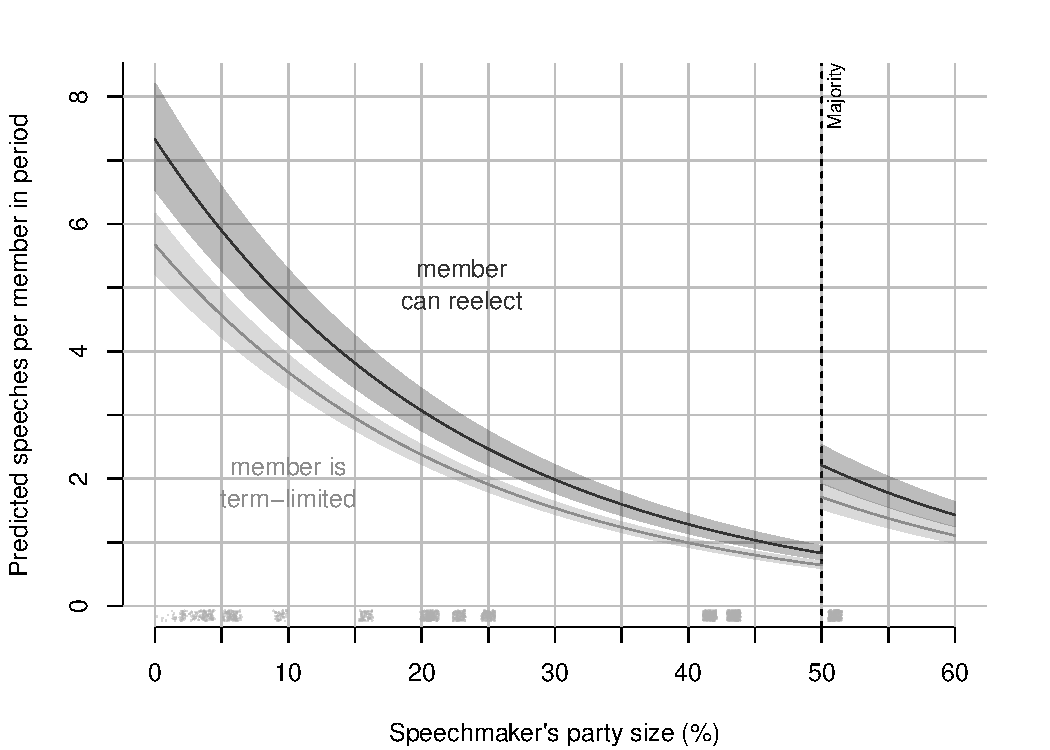
\includegraphics[width=.67\columnwidth]{../plots/predictedWords.pdf}
    \caption{Predicted speech length. Lines report point predictions using model 5.}\label{F:predict}
\end{figure}




\begin{figure}
  \centering
    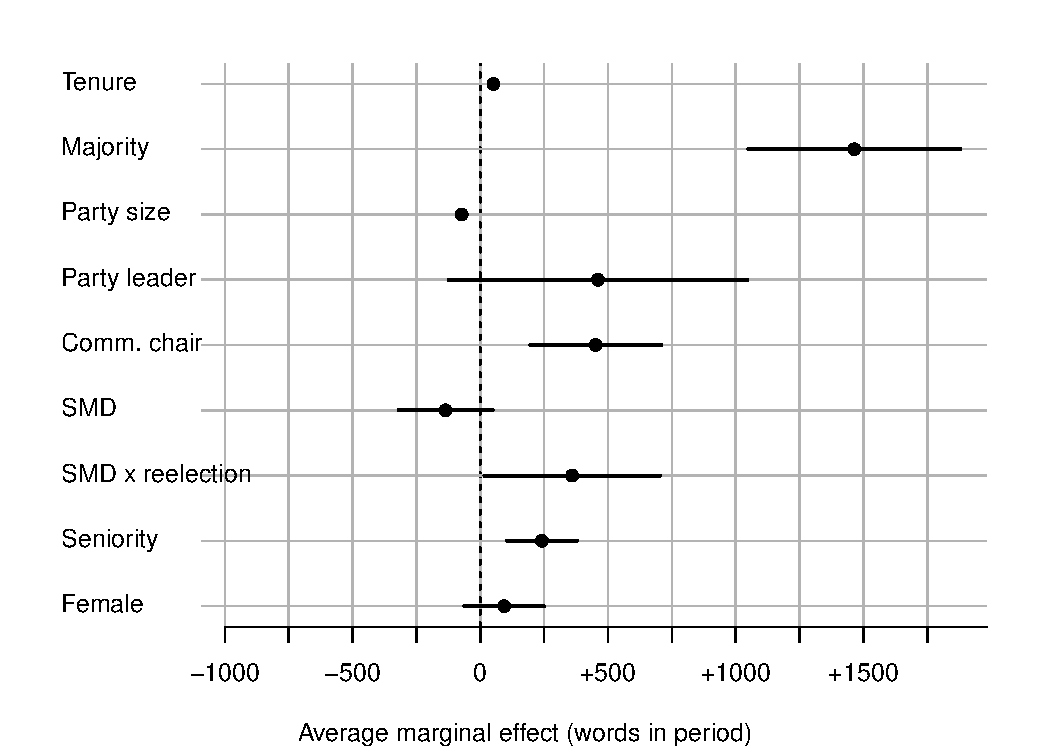
\includegraphics[width=.67\columnwidth]{../plots/avgMgEffects.pdf}
    \caption{Average marginal effects from model 5. Dots report the effect in expected period speech length of a unit change in each independent variable, all else at mean values; bars are 95-percent confidence intervals.}\label{F:avgmgeff}
\end{figure}

%% model 5 (fit2 in code) average marginal effects
%%      factor       AME       SE        z      p     lower     upper
%%  ev.pot.dys   51.3100   2.6546  19.3285 0.0000   46.1070   56.5129
%%        dmaj 1464.4438 211.4850   6.9246 0.0000 1049.9408 1878.9469
%%    size.maj  -72.7583   4.9124 -14.8113 0.0000  -82.3863  -63.1303
%%     dleader  460.6492 298.1915   1.5448 0.1224 -123.7954 1045.0937
%%      dchair  451.9050 130.7671   3.4558 0.0005  195.6061  708.2039
%%        dsmd -135.7903  93.9759  -1.4449 0.1485 -319.9796   48.3991
%%      dsmd64  359.7821 175.2500   2.0530 0.0401   16.2985  703.2657
%%   seniority  241.5023  69.7417   3.4628 0.0005  104.8111  378.1935
%%        dfem   93.4748  79.3548   1.1779 0.2388  -62.0578  249.0074
%%        dsup -507.2173 160.3330  -3.1635 0.0016 -821.4642 -192.9703
%%         d62  259.0260  89.6724   2.8886 0.0039   83.2712  434.7807
%%         d64 -132.3693 165.2884  -0.8008 0.4232 -456.3285  191.5899

Figure \ref{F:avgmgeff} reports changes in the average predicted number of words associated with unit changes in explanatory variables. This exercise uses model 5 estimates. By translating into interpretable quantities, marginal effects are a convenient way to gauge negative binomial regression coefficients. It is clear in the plot that the larges effect is attributable to majority status. Other things constant (at mean values), members in the majority party each spoke between about 1,000 and 1,900 more words per period than the rest of the chamber. Multiplication of that average by Morena's 254 members in the 64th Legislature produces 372 thousand additional words---47 percent of all words in the median ordinary period.

%% The report from a committee with a coalition chair experiences a 0.17
%% hike (0.06 standard error) in the likelihood of receiving a closed rule compared to a report by an
%% opposition-chaired committee. The effect is as big as the average marginal effects of Hacienda
%% Referral (0.18), which capures mostly high-significance draft laws, and that of Multiple Referrals
%% (0.16), which we view as an indicator of issue complexity. We therefore find no statistical evidence
%% to reject our Hypothesis 1. The results also confirm hypothesis 2, showing that a bill reported by a
%% generally less friendly committe (chaired by the opposition), has a higher probability of receiving
%% an open rule on the floor, thereby allowing the floor majority to bring back the bill to the median
%% through floor amendments. Thus, presidents use open rules to control bills coming from preference
%% distant committee chairs.
%% The substantial effects of Hacienda Referral and Multiple Referrals deserve comment. They
%% suggest, first, that when spending gets in the way, restrictive rules are the norm in Chile. Recall
%% that Multiple Referrals exclude the Finance Committee, so there is an independent effect of bills
%% with jurisdictional overlaps worth investigating further, and which must be associated, in part at
%% least, to influencing the report through a friendlier committee. 16 Furthermore, note that the Finance
%% Committee was always chaired by a coalition member but, with the exception of the 1998–2000
%% period, never by a co-partisan of the president. This may explain the milder effect of the partisan
%% specification of our key variable in model 1.
%% Another effect worth highlighting is Introd. in Senate. Bills successfully passing the Upper
%% Chamber first, where the opposition was systematically larger and attimes in control, were much
%% less likely to get urgent status (the average marginal effect is −0.15 and significant). This suggests
%% that agreements and compromises reached in the Senate ignited less, not more, protection from
%% floor amendments in the Cámara’s plenary, most likely as a consequence of the greater prefer-
%% ence divergence between the President and the opposition-led Senate. Analysis of inter-chamber
%% negotiation and the reliance on urgency in the Upper Chamber are interesting venues for future
%% research.
%% Finally, there are time trends in fast-track authority that simulations reveal neatly. Figure 5
%% portrays the predicted probability that a bill enters the fast-track throughout the legislative year.
%% Regressors in model 3 are held constant to simulate a bill sent to the Cámara in the 2006–10
%% Legislature that was referred to a single committee, excluding Hacienda. Presidential Approval
%% (insignificant across models) is set to the mean for President Bachelet’s first term, coinciding in full
%% with the 2006–10 Legislature. The inverted-U shape shows how fast-track probability, predicted
%% at 0.17 for coalition-chaired committees at the start, and 0.08 for the rest, becomes much likelier
%% in the first half of the legislative year. By the second quarter (June–August), the probability is at
%% its peak, about 0.32 percent and 0.17, respectively. It then experiences a sharp drop, ending the
%% austral Summer break at 0.13 for coalition-chaired committees, and 0.05 for others. And while 95-
%% percent confidence bands overlap, they barely do so at the middle of the legislative year, lending
%% confidence that we are picking up a signal and not just random noise.

    \subsubsection{Predicted words}


  
\section{Country-Specific Section} [ca 1000 words]
In this section, you can feel free to make model extensions that have interest in the light of the chapter you are exploring. Please do not forget to explain the variables in use, as well as why they are important for your country. Include a table of results plus a plot for marginal effects. 

\section{Conclusions} [ca 500 words]
concluding discussion of general patterns of speechmaking (institutions and empirical results in terms of background variables)


Stuff to add to EMM’s text
DONE 3. In terms of window of observation/time period under study: we don’t have a particular guideline for this. Please use the window of observation that you believe is more representative of the politics of legislative debate in your country. Ideally we would like each chapter to include several legislative periods, but we are pragmatic here, considering data availability.
EMM: Terminology
- A Legislature (with Roman numerals for reasons I ignore) is an elected chamber for a legislative term, called a Congress in the U.S. Concurrent with presidential elections the chamber of deputies renovates in whole, and again at the presidential mid-term. Diputados remain three years in office and were single term-limited up to 2021. The 2021 mid-term election will be the first since 1932 to allow incumbents on the ballot, a major change in Mexican legislative politics.
- Legislative years break into two "ordinary periods", one covering the months of September through December, inclusive, another February through April, also inclusive. "Extraordinary periods" may be convened during the recess in order to consider a specific bill. Analysis aggregates each member's speeches in the duration of a given period (merging together all extraordinary periods that year, if any). So members in a legislative year like 2012-13 (that had no extraordinary periods) have two word aggregates in the dataset, one for each ordinary period; in a year like 2013-14 (that did), they have three word aggregates in the data. Periods are the units of aggregation in the analysis. 
- A plenary session is a specific date in the calendar when diputados met. During ordinary periods, sessions are usually held on Tuesdays and Thursdays, and may be scheduled in other weekdays if the Jucopo so decides. Diputados met on forty and thirty-one days in the first and second ordinary periods of 2013-14, respectively, and nine days in extraordinary periods, for a yearly total of eighty session days. (A session in North-American legislative parlance is a Mexican period.)

\section{Appendix: Terminology}

\singlespacing

- A *Legislature* is an elected chamber for a legislative term, called a Congress in the U.S. Concurrent with presidential elections the chamber of deputies renovates in whole, and again at the presidential mid-term. Diputados remain three years in office and were single term-limited up to 2021. The 2021 mid-term election will be the first since 1932 to allow incumbents on the ballot, a major change in Mexican legislative politics. Analysis includes the 60th, 62nd, and 64th Legislatures (the Mexican Congress relies on Roman numerals to distinguish Legislatures since the second half of the Nineteenth century).

- Legislative years break into two *ordinary legislative periods*, one covering the months of September through December, inclusive, another February through April, also inclusive. *Extraordinary legislative periods* may be convened during the recess in order to consider a specific bill. Analysis aggregates each member's speeches in the duration of a given period (merging together all extraordinary periods that year, if any). So members in a legislative year like 2012-13 (that had no extraordinary periods) have two word aggregates in the dataset, one for each ordinary period; in a year like 2013-14 (that did), they have three word aggregates in the data. Periods are the units of observation in the analysis. 

- A *plenary session* (or simply a session) is a specific date in the calendar when diputados met. During ordinary periods, sessions are usually held on Tuesdays and Thursdays, and may be scheduled in other weekdays if the Jucopo so decides. Diputados met on forty and thirty-one days in the first and second ordinary periods of 2013-14, respectively, and nine days in extraordinary periods, for a yearly total of eighty session days. (A session in North-American legislative parlance is a Mexican period.)

\newpage

\section*{Acknowledgements}
Eric Magar received financial support from the Asociaci\'on Mexicana de Cultura \textsc{a.c.}\ and \textsc{conacyt}'s Sistema Nacional de Investigadores. The author is grateful to Ana Lucía Enríquez, Eugenio Solís Flores, Vidal, Sonia Kuri for research assistance. The author is responsible for mistakes and shortcomings in the study.

%\listofendnotes

\bibliographystyle{apsr}

\bibliography{../bib/magar}

%% \begin{thebibliography}{xx}

%% \harvarditem{Alem\'an \harvardand\ Tsebelis}{2016}{aleman-tsebelis-2016-book}
%% Alem\'an, Eduardo \harvardand\ George Tsebelis. 2016.
%% \newblock {\em Legislative Institutions and Lawmaking in Latin America}.
%% \newblock Oxford:  Oxford University Press.

%% \harvarditem{Alem\'an \harvardand\ Navia}{2009}{aleman.navia.UrgChi.2009}
%% Alem\'an, Eduardo \harvardand\ Patricio Navia. 2009.
%% \newblock ``Institutions and the Legislative Success of `Strong' Presidents: An
%%   Analysis of Government Bills in {Chile}.'' {\em Journal of Legislative
%%   Studies} 15(4):401--19.

%% \end{thebibliography}


\end{document}

